\documentclass[ExampleMasters.tex]{subfiles}
\begin{document}
\chapter{Optimisation Results}

\section{Introduction}
	As set out in the abstract, the generic vehicle model described in the Chapter 4 is used in consonance with the genetic algorithm described in Chapter 2 to derive optimal vehicle propulsion configurations for years 2015, 2020, 2025 and 2030, the objective function optimised being the vehicle productivity over the lifetime of the first owner's holding.\\

	In this chapter, the results of the optimisation shall be presented in four different sub-sections. The first contains a brief listing of the results derived from successive runs of the genetic algorithm lasting 100 generations each. The following subsections are an analysis of the results in different headings.

\section{Overview of the results}
	Optimal axle propulsion configurations are derived for the years specified above. The following tables list the results for varying gross combination weights of 50t, 60t, 70t and 80t for each of the four years in succession.

	\begin{table}[H]
		\caption{Optimal combination configurations - Year 2015}
		\centering
		\begin{tabular}{c c c}
		\hline\hline
		GCW & Optimal configuration & Vehicle Productivity \\  
		\hline
		50 & 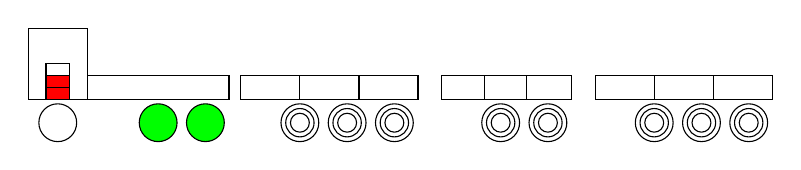
\begin{tikzpicture}[ scale=0.3]
				% Tractor
				\draw (7.5,2) rectangle (10,5);
				\draw[fill=red] (8.25,2) rectangle (9.25,2.5);
				\draw[fill=red] (8.25,2.5) rectangle (9.25,3);
				\draw (8.25,3) rectangle (9.25,3.5);
				\draw (10,2) rectangle (16,3);
				\draw (8.75,1) circle (0.8);
				\draw[fill=green!100] (13,1) circle (0.8);
				\draw[fill=green!100] (15,1) circle (0.8);

				% Semi-trailer
				\draw (16.5,2) rectangle (19,3);
				\draw (19,2) rectangle (21.5,3);
				\draw (21.5,2) rectangle (24,3);
				% \draw (17,0.5) rectangle (18,1);
				% \draw (17,1) rectangle (18,1.5);
				% \draw (17,1.5) rectangle (18,2);
				\draw (19,1) circle (0.8);
				\draw (19,1) circle (0.6);
				\draw (19,1) circle (0.4);
				\draw (21,1) circle (0.8);
				\draw (21,1) circle (0.6);
				\draw (21,1) circle (0.4);	
				\draw (23,1) circle (0.8);
				\draw (23,1) circle (0.6);
				\draw (23,1) circle (0.4);

				% Dolly
				\draw (25,2) rectangle (26.8,3);
				\draw (26.8,2) rectangle (28.6,3);
				\draw (28.6,2) rectangle (30.5,3);
				% \draw (25.5,0.5) rectangle (26.5,1);
				% \draw (25.5,1) rectangle (26.5,1.5);
				% \draw (25.5,1.5) rectangle (26.5,2);
				\draw (27.5,1) circle (0.8);
				\draw (27.5,1) circle (0.6);
				\draw (27.5,1) circle (0.4);	
				\draw (29.5,1) circle (0.8);
				\draw (29.5,1) circle (0.6);
				\draw (29.5,1) circle (0.4);	

				% Semi-trailer
				\draw (31.5,2) rectangle (34,3);
				\draw (34,2) rectangle (36.5,3);
				\draw (36.5,2) rectangle (39,3);
				% \draw (32,0.5) rectangle (33,1);
				% \draw (32,1) rectangle (33,1.5);
				% \draw (32,1.5) rectangle (33,2);
				\draw (34,1) circle (0.8);
				\draw (34,1) circle (0.6);
				\draw (34,1) circle (0.4);
				\draw (36,1) circle (0.8);
				\draw (36,1) circle (0.6);
				\draw (36,1) circle (0.4);	
				\draw (38,1) circle (0.8);
				\draw (38,1) circle (0.6);
				\draw (38,1) circle (0.4);
			\end{tikzpicture} & 0.960028 \\

		60 & 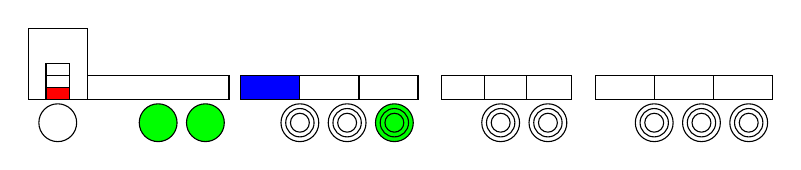
\begin{tikzpicture}[ scale=0.3]
				% Tractor
				\draw (7.5,2) rectangle (10,5);
				\draw[fill=red] (8.25,2) rectangle (9.25,2.5);
				\draw (8.25,2.5) rectangle (9.25,3);
				\draw (8.25,3) rectangle (9.25,3.5);
				\draw (10,2) rectangle (16,3);
				\draw (8.75,1) circle (0.8);
				\draw[fill=green!100] (13,1) circle (0.8);
				\draw[fill=green!100] (15,1) circle (0.8);

				% Semi-trailer
				\draw[fill=blue] (16.5,2) rectangle (19,3);
				\draw (19,2) rectangle (21.5,3);
				\draw (21.5,2) rectangle (24,3);
				% \draw (17,0.5) rectangle (18,1);
				% \draw (17,1) rectangle (18,1.5);
				% \draw (17,1.5) rectangle (18,2);
				\draw (19,1) circle (0.8);
				\draw (19,1) circle (0.6);
				\draw (19,1) circle (0.4);
				\draw (21,1) circle (0.8);
				\draw (21,1) circle (0.6);
				\draw (21,1) circle (0.4);	
				\draw[fill=green!100] (23,1) circle (0.8);
				\draw (23,1) circle (0.6);
				\draw (23,1) circle (0.4);

				% Dolly
				\draw (25,2) rectangle (26.8,3);
				\draw (26.8,2) rectangle (28.6,3);
				\draw (28.6,2) rectangle (30.5,3);
				% \draw (25.5,0.5) rectangle (26.5,1);
				% \draw (25.5,1) rectangle (26.5,1.5);
				% \draw (25.5,1.5) rectangle (26.5,2);
				\draw (27.5,1) circle (0.8);
				\draw (27.5,1) circle (0.6);
				\draw (27.5,1) circle (0.4);	
				\draw (29.5,1) circle (0.8);
				\draw (29.5,1) circle (0.6);
				\draw (29.5,1) circle (0.4);	

				% Semi-trailer
				\draw (31.5,2) rectangle (34,3);
				\draw (34,2) rectangle (36.5,3);
				\draw (36.5,2) rectangle (39,3);
				% \draw (32,0.5) rectangle (33,1);
				% \draw (32,1) rectangle (33,1.5);
				% \draw (32,1.5) rectangle (33,2);
				\draw (34,1) circle (0.8);
				\draw (34,1) circle (0.6);
				\draw (34,1) circle (0.4);
				\draw (36,1) circle (0.8);
				\draw (36,1) circle (0.6);
				\draw (36,1) circle (0.4);	
				\draw (38,1) circle (0.8);
				\draw (38,1) circle (0.6);
				\draw (38,1) circle (0.4);
			\end{tikzpicture} & 1.25954 \\

		70 & 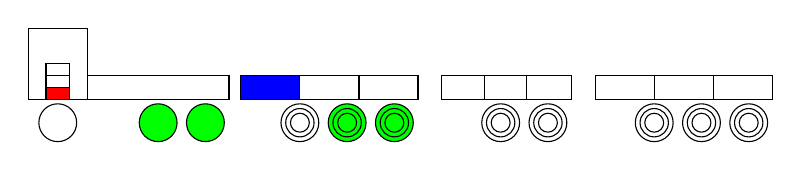
\begin{tikzpicture}[ scale=0.3]
				% Tractor
				\draw (7.5,2) rectangle (10,5);
				\draw[fill=red] (8.25,2) rectangle (9.25,2.5);
				\draw (8.25,2.5) rectangle (9.25,3);
				\draw (8.25,3) rectangle (9.25,3.5);
				\draw (10,2) rectangle (16,3);
				\draw (8.75,1) circle (0.8);
				\draw[fill=green!100] (13,1) circle (0.8);
				\draw[fill=green!100] (15,1) circle (0.8);

				% Semi-trailer
				\draw[fill=blue] (16.5,2) rectangle (19,3);
				\draw (19,2) rectangle (21.5,3);
				\draw (21.5,2) rectangle (24,3);
				% \draw (17,0.5) rectangle (18,1);
				% \draw (17,1) rectangle (18,1.5);
				% \draw (17,1.5) rectangle (18,2);
				\draw (19,1) circle (0.8);
				\draw (19,1) circle (0.6);
				\draw (19,1) circle (0.4);
				\draw[fill=green!100] (21,1) circle (0.8);
				\draw (21,1) circle (0.6);
				\draw (21,1) circle (0.4);	
				\draw[fill=green!100] (23,1) circle (0.8);
				\draw (23,1) circle (0.6);
				\draw (23,1) circle (0.4);

				% Dolly
				\draw (25,2) rectangle (26.8,3);
				\draw (26.8,2) rectangle (28.6,3);
				\draw (28.6,2) rectangle (30.5,3);
				% \draw (25.5,0.5) rectangle (26.5,1);
				% \draw (25.5,1) rectangle (26.5,1.5);
				% \draw (25.5,1.5) rectangle (26.5,2);
				\draw (27.5,1) circle (0.8);
				\draw (27.5,1) circle (0.6);
				\draw (27.5,1) circle (0.4);	
				\draw (29.5,1) circle (0.8);
				\draw (29.5,1) circle (0.6);
				\draw (29.5,1) circle (0.4);	

				% Semi-trailer
				\draw (31.5,2) rectangle (34,3);
				\draw (34,2) rectangle (36.5,3);
				\draw (36.5,2) rectangle (39,3);
				% \draw (32,0.5) rectangle (33,1);
				% \draw (32,1) rectangle (33,1.5);
				% \draw (32,1.5) rectangle (33,2);
				\draw (34,1) circle (0.8);
				\draw (34,1) circle (0.6);
				\draw (34,1) circle (0.4);
				\draw (36,1) circle (0.8);
				\draw (36,1) circle (0.6);
				\draw (36,1) circle (0.4);	
				\draw (38,1) circle (0.8);
				\draw (38,1) circle (0.6);
				\draw (38,1) circle (0.4);
			\end{tikzpicture} & 1.49906 \\
		
		80 & 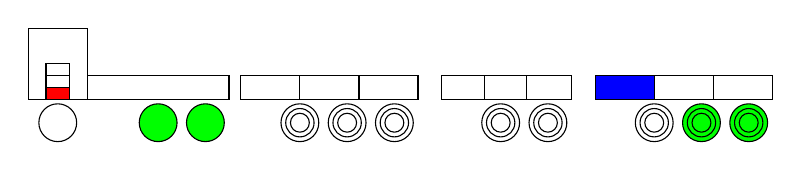
\begin{tikzpicture}[ scale=0.3]
				% Tractor
				\draw (7.5,2) rectangle (10,5);
				\draw[fill=red] (8.25,2) rectangle (9.25,2.5);
				\draw (8.25,2.5) rectangle (9.25,3);
				\draw (8.25,3) rectangle (9.25,3.5);
				\draw (10,2) rectangle (16,3);
				\draw (8.75,1) circle (0.8);
				\draw[fill=green!100] (13,1) circle (0.8);
				\draw[fill=green!100] (15,1) circle (0.8);

				% Semi-trailer
				\draw (16.5,2) rectangle (19,3);
				\draw (19,2) rectangle (21.5,3);
				\draw (21.5,2) rectangle (24,3);
				% \draw (17,0.5) rectangle (18,1);
				% \draw (17,1) rectangle (18,1.5);
				% \draw (17,1.5) rectangle (18,2);
				\draw (19,1) circle (0.8);
				\draw (19,1) circle (0.6);
				\draw (19,1) circle (0.4);
				\draw (21,1) circle (0.8);
				\draw (21,1) circle (0.6);
				\draw (21,1) circle (0.4);	
				\draw (23,1) circle (0.8);
				\draw (23,1) circle (0.6);
				\draw (23,1) circle (0.4);

				% Dolly
				\draw (25,2) rectangle (26.8,3);
				\draw (26.8,2) rectangle (28.6,3);
				\draw (28.6,2) rectangle (30.5,3);
				% \draw (25.5,0.5) rectangle (26.5,1);
				% \draw (25.5,1) rectangle (26.5,1.5);
				% \draw (25.5,1.5) rectangle (26.5,2);
				\draw (27.5,1) circle (0.8);
				\draw (27.5,1) circle (0.6);
				\draw (27.5,1) circle (0.4);	
				\draw (29.5,1) circle (0.8);
				\draw (29.5,1) circle (0.6);
				\draw (29.5,1) circle (0.4);	

				% Semi-trailer
				\draw[fill=blue] (31.5,2) rectangle (34,3);
				\draw (34,2) rectangle (36.5,3);
				\draw (36.5,2) rectangle (39,3);
				% \draw (32,0.5) rectangle (33,1);
				% \draw (32,1) rectangle (33,1.5);
				% \draw (32,1.5) rectangle (33,2);
				\draw (34,1) circle (0.8);
				\draw (34,1) circle (0.6);
				\draw (34,1) circle (0.4);
				\draw[fill=green!100] (36,1) circle (0.8);
				\draw (36,1) circle (0.6);
				\draw (36,1) circle (0.4);	
				\draw[fill=green!100] (38,1) circle (0.8);
				\draw (38,1) circle (0.6);
				\draw (38,1) circle (0.4);
			\end{tikzpicture} & 1.80818 \\
			\hline
		\end{tabular}
		\label{table:optVisComb2015}
	\end{table}

	\begin{table}[H]
		\caption{Optimal combination configurations - Year 2015}
		\centering
		\begin{tabular}{c c c c c c}
		\hline\hline
		GCW & \multicolumn{4}{c}{Optimal configuration} & Vehicle Productivity \\ \cline{2-5}
		(t) & Tractor & Semi-trailer & Dolly & Semi-trailer & (\euro/\euro)\\ 
		\hline
		50 & 010\textbackslash000\textbackslash011 &
			 001\textbackslash001\textbackslash000 & 100\textbackslash001\textbackslash00 &
			 100\textbackslash001\textbackslash000 & 0.960028 \\
		60 & 100\textbackslash000\textbackslash011 &
			 001\textbackslash100\textbackslash001 & 010\textbackslash010\textbackslash00 &
			 010\textbackslash100\textbackslash000 & 1.25954 \\
		70 & 100\textbackslash000\textbackslash011 & 
			 001\textbackslash100\textbackslash110 & 010\textbackslash001\textbackslash00  & 
			 100\textbackslash010\textbackslash000 & 1.49906 \\
		80 & 100\textbackslash000\textbackslash011 &
			 100\textbackslash010\textbackslash000 & 100\textbackslash100\textbackslash00 &
			 001\textbackslash100\textbackslash011 & 1.80818 \\
		\hline
		\end{tabular}
		\label{table:optComb2015}
	\end{table}

	\begin{table}[H]
		\caption{Optimal combination configurations - Year 2020}
		\centering
		\begin{tabular}{c c c}
		\hline\hline
		GCW & Optimal configuration & Vehicle Productivity \\  
		\hline
		50 & 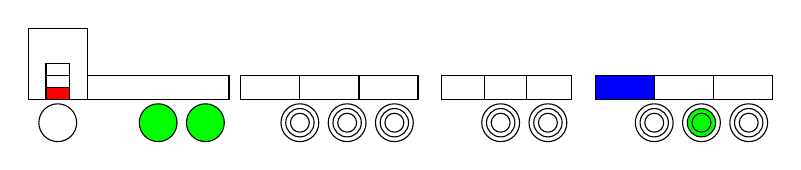
\begin{tikzpicture}[ scale=0.3]
				% Tractor
				\draw (7.5,2) rectangle (10,5);
				\draw[fill=red] (8.25,2) rectangle (9.25,2.5);
				\draw (8.25,2.5) rectangle (9.25,3);
				\draw (8.25,3) rectangle (9.25,3.5);
				\draw (10,2) rectangle (16,3);
				\draw (8.75,1) circle (0.8);
				\draw[fill=green!100] (13,1) circle (0.8);
				\draw[fill=green!100] (15,1) circle (0.8);

				% Semi-trailer
				\draw (16.5,2) rectangle (19,3);
				\draw (19,2) rectangle (21.5,3);
				\draw (21.5,2) rectangle (24,3);
				% \draw (17,0.5) rectangle (18,1);
				% \draw (17,1) rectangle (18,1.5);
				% \draw (17,1.5) rectangle (18,2);
				\draw (19,1) circle (0.8);
				\draw (19,1) circle (0.6);
				\draw (19,1) circle (0.4);
				\draw (21,1) circle (0.8);
				\draw (21,1) circle (0.6);
				\draw (21,1) circle (0.4);	
				\draw (23,1) circle (0.8);
				\draw (23,1) circle (0.6);
				\draw (23,1) circle (0.4);

				% Dolly
				\draw (25,2) rectangle (26.8,3);
				\draw (26.8,2) rectangle (28.6,3);
				\draw (28.6,2) rectangle (30.5,3);
				% \draw (25.5,0.5) rectangle (26.5,1);
				% \draw (25.5,1) rectangle (26.5,1.5);
				% \draw (25.5,1.5) rectangle (26.5,2);
				\draw (27.5,1) circle (0.8);
				\draw (27.5,1) circle (0.6);
				\draw (27.5,1) circle (0.4);	
				\draw (29.5,1) circle (0.8);
				\draw (29.5,1) circle (0.6);
				\draw (29.5,1) circle (0.4);	

				% Semi-trailer
				\draw[fill=blue] (31.5,2) rectangle (34,3);
				\draw (34,2) rectangle (36.5,3);
				\draw (36.5,2) rectangle (39,3);
				% \draw (32,0.5) rectangle (33,1);
				% \draw (32,1) rectangle (33,1.5);
				% \draw (32,1.5) rectangle (33,2);
				\draw (34,1) circle (0.8);
				\draw (34,1) circle (0.6);
				\draw (34,1) circle (0.4);
				\draw (36,1) circle (0.8);
				\draw[fill=green!100] (36,1) circle (0.6);
				\draw (36,1) circle (0.4);	
				\draw (38,1) circle (0.8);
				\draw (38,1) circle (0.6);
				\draw (38,1) circle (0.4);
			\end{tikzpicture} & 0.974871 \\

		60 & 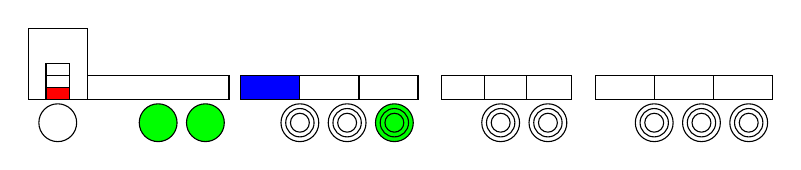
\begin{tikzpicture}[ scale=0.3]
				% Tractor
				\draw (7.5,2) rectangle (10,5);
				\draw[fill=red] (8.25,2) rectangle (9.25,2.5);
				\draw (8.25,2.5) rectangle (9.25,3);
				\draw (8.25,3) rectangle (9.25,3.5);
				\draw (10,2) rectangle (16,3);
				\draw (8.75,1) circle (0.8);
				\draw[fill=green!100] (13,1) circle (0.8);
				\draw[fill=green!100] (15,1) circle (0.8);

				% Semi-trailer
				\draw[fill=blue] (16.5,2) rectangle (19,3);
				\draw (19,2) rectangle (21.5,3);
				\draw (21.5,2) rectangle (24,3);
				% \draw (17,0.5) rectangle (18,1);
				% \draw (17,1) rectangle (18,1.5);
				% \draw (17,1.5) rectangle (18,2);
				\draw (19,1) circle (0.8);
				\draw (19,1) circle (0.6);
				\draw (19,1) circle (0.4);
				\draw (21,1) circle (0.8);
				\draw (21,1) circle (0.6);
				\draw (21,1) circle (0.4);	
				\draw[fill=green!100] (23,1) circle (0.8);
				\draw (23,1) circle (0.6);
				\draw (23,1) circle (0.4);

				% Dolly
				\draw (25,2) rectangle (26.8,3);
				\draw (26.8,2) rectangle (28.6,3);
				\draw (28.6,2) rectangle (30.5,3);
				% \draw (25.5,0.5) rectangle (26.5,1);
				% \draw (25.5,1) rectangle (26.5,1.5);
				% \draw (25.5,1.5) rectangle (26.5,2);
				\draw (27.5,1) circle (0.8);
				\draw (27.5,1) circle (0.6);
				\draw (27.5,1) circle (0.4);	
				\draw (29.5,1) circle (0.8);
				\draw (29.5,1) circle (0.6);
				\draw (29.5,1) circle (0.4);	

				% Semi-trailer
				\draw (31.5,2) rectangle (34,3);
				\draw (34,2) rectangle (36.5,3);
				\draw (36.5,2) rectangle (39,3);
				% \draw (32,0.5) rectangle (33,1);
				% \draw (32,1) rectangle (33,1.5);
				% \draw (32,1.5) rectangle (33,2);
				\draw (34,1) circle (0.8);
				\draw (34,1) circle (0.6);
				\draw (34,1) circle (0.4);
				\draw (36,1) circle (0.8);
				\draw (36,1) circle (0.6);
				\draw (36,1) circle (0.4);	
				\draw (38,1) circle (0.8);
				\draw (38,1) circle (0.6);
				\draw (38,1) circle (0.4);
			\end{tikzpicture} & 1.27334 \\

		70 & 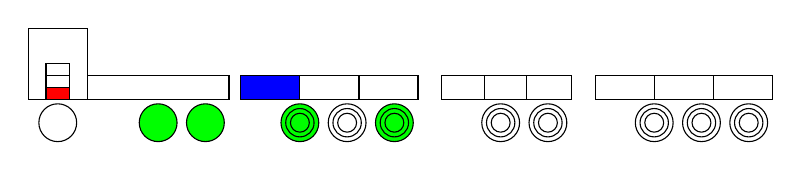
\begin{tikzpicture}[ scale=0.3]
				% Tractor
				\draw (7.5,2) rectangle (10,5);
				\draw[fill=red] (8.25,2) rectangle (9.25,2.5);
				\draw (8.25,2.5) rectangle (9.25,3);
				\draw (8.25,3) rectangle (9.25,3.5);
				\draw (10,2) rectangle (16,3);
				\draw (8.75,1) circle (0.8);
				\draw[fill=green!100] (13,1) circle (0.8);
				\draw[fill=green!100] (15,1) circle (0.8);

				% Semi-trailer
				\draw[fill=blue] (16.5,2) rectangle (19,3);
				\draw (19,2) rectangle (21.5,3);
				\draw (21.5,2) rectangle (24,3);
				% \draw (17,0.5) rectangle (18,1);
				% \draw (17,1) rectangle (18,1.5);
				% \draw (17,1.5) rectangle (18,2);
				\draw[fill=green!100] (19,1) circle (0.8);
				\draw (19,1) circle (0.6);
				\draw (19,1) circle (0.4);
				\draw (21,1) circle (0.8);
				\draw (21,1) circle (0.6);
				\draw (21,1) circle (0.4);	
				\draw[fill=green!100] (23,1) circle (0.8);
				\draw (23,1) circle (0.6);
				\draw (23,1) circle (0.4);

				% Dolly
				\draw (25,2) rectangle (26.8,3);
				\draw (26.8,2) rectangle (28.6,3);
				\draw (28.6,2) rectangle (30.5,3);
				% \draw (25.5,0.5) rectangle (26.5,1);
				% \draw (25.5,1) rectangle (26.5,1.5);
				% \draw (25.5,1.5) rectangle (26.5,2);
				\draw (27.5,1) circle (0.8);
				\draw (27.5,1) circle (0.6);
				\draw (27.5,1) circle (0.4);	
				\draw (29.5,1) circle (0.8);
				\draw (29.5,1) circle (0.6);
				\draw (29.5,1) circle (0.4);	

				% Semi-trailer
				\draw (31.5,2) rectangle (34,3);
				\draw (34,2) rectangle (36.5,3);
				\draw (36.5,2) rectangle (39,3);
				% \draw (32,0.5) rectangle (33,1);
				% \draw (32,1) rectangle (33,1.5);
				% \draw (32,1.5) rectangle (33,2);
				\draw (34,1) circle (0.8);
				\draw (34,1) circle (0.6);
				\draw (34,1) circle (0.4);
				\draw (36,1) circle (0.8);
				\draw (36,1) circle (0.6);
				\draw (36,1) circle (0.4);	
				\draw (38,1) circle (0.8);
				\draw (38,1) circle (0.6);
				\draw (38,1) circle (0.4);
			\end{tikzpicture} & 1.51884 \\
		
		80 & 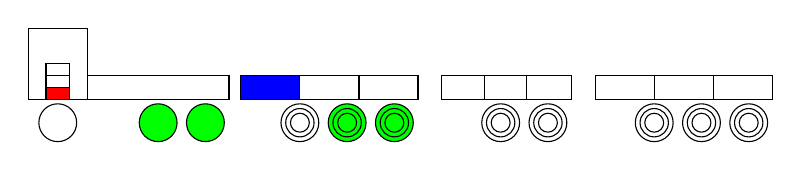
\begin{tikzpicture}[ scale=0.3]
				% Tractor
				\draw (7.5,2) rectangle (10,5);
				\draw[fill=red] (8.25,2) rectangle (9.25,2.5);
				\draw (8.25,2.5) rectangle (9.25,3);
				\draw (8.25,3) rectangle (9.25,3.5);
				\draw (10,2) rectangle (16,3);
				\draw (8.75,1) circle (0.8);
				\draw[fill=green!100] (13,1) circle (0.8);
				\draw[fill=green!100] (15,1) circle (0.8);

				% Semi-trailer
				\draw[fill=blue] (16.5,2) rectangle (19,3);
				\draw (19,2) rectangle (21.5,3);
				\draw (21.5,2) rectangle (24,3);
				% \draw (17,0.5) rectangle (18,1);
				% \draw (17,1) rectangle (18,1.5);
				% \draw (17,1.5) rectangle (18,2);
				\draw (19,1) circle (0.8);
				\draw (19,1) circle (0.6);
				\draw (19,1) circle (0.4);
				\draw[fill=green!100] (21,1) circle (0.8);
				\draw (21,1) circle (0.6);
				\draw (21,1) circle (0.4);	
				\draw[fill=green!100] (23,1) circle (0.8);
				\draw (23,1) circle (0.6);
				\draw (23,1) circle (0.4);

				% Dolly
				\draw (25,2) rectangle (26.8,3);
				\draw (26.8,2) rectangle (28.6,3);
				\draw (28.6,2) rectangle (30.5,3);
				% \draw (25.5,0.5) rectangle (26.5,1);
				% \draw (25.5,1) rectangle (26.5,1.5);
				% \draw (25.5,1.5) rectangle (26.5,2);
				\draw (27.5,1) circle (0.8);
				\draw (27.5,1) circle (0.6);
				\draw (27.5,1) circle (0.4);	
				\draw (29.5,1) circle (0.8);
				\draw (29.5,1) circle (0.6);
				\draw (29.5,1) circle (0.4);	

				% Semi-trailer
				\draw (31.5,2) rectangle (34,3);
				\draw (34,2) rectangle (36.5,3);
				\draw (36.5,2) rectangle (39,3);
				% \draw (32,0.5) rectangle (33,1);
				% \draw (32,1) rectangle (33,1.5);
				% \draw (32,1.5) rectangle (33,2);
				\draw (34,1) circle (0.8);
				\draw (34,1) circle (0.6);
				\draw (34,1) circle (0.4);
				\draw (36,1) circle (0.8);
				\draw (36,1) circle (0.6);
				\draw (36,1) circle (0.4);	
				\draw (38,1) circle (0.8);
				\draw (38,1) circle (0.6);
				\draw (38,1) circle (0.4);
			\end{tikzpicture} & 1.83086 \\
			\hline
		\end{tabular}
		\label{table:optVisComb2020}
	\end{table}

	\begin{table}[H]
		\caption{Optimal combination configurations - Year 2020}
		\centering
		\begin{tabular}{c c c c c c}
		\hline\hline
		GCW & \multicolumn{4}{c}{Optimal configuration} & Vehicle Productivity \\ \cline{2-5}
		(t) & Tractor & Semi-trailer & Dolly & Semi-trailer & (\euro/\euro)\\ 
		\hline
		50 & 100\textbackslash000\textbackslash011 &
			 100\textbackslash100\textbackslash000  & 001\textbackslash001\textbackslash00  & 
			 001\textbackslash100\textbackslash010 & 0.974871 \\
		60 & 100\textbackslash000\textbackslash011 & 
			 001\textbackslash100\textbackslash001 & 100\textbackslash010\textbackslash00 &
			 100\textbackslash010\textbackslash000 & 1.27334 \\
		70 & 100\textbackslash000\textbackslash011 &
			 001\textbackslash100\textbackslash101 & 100\textbackslash100\textbackslash00 &
			 001\textbackslash010\textbackslash000 & 1.49906 \\
		80 & 100\textbackslash000\textbackslash011 & 
			 001\textbackslash100\textbackslash011 & 010\textbackslash100\textbackslash00 &
			 001\textbackslash001\textbackslash000 & 1.80818 \\
		\hline
		\end{tabular}
		\label{table:optComb2020}
	\end{table}

	\begin{table}[H]
		\caption{Optimal combination configurations - Year 2025}
		\centering
		\begin{tabular}{c c c}
		\hline\hline
		GCW & Optimal configuration & Vehicle Productivity \\  
		\hline
		50 & 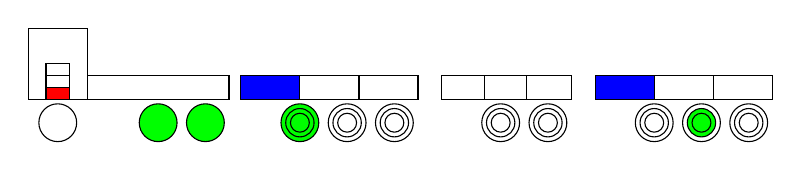
\begin{tikzpicture}[ scale=0.3]
				% Tractor
				\draw (7.5,2) rectangle (10,5);
				\draw[fill=red] (8.25,2) rectangle (9.25,2.5);
				\draw (8.25,2.5) rectangle (9.25,3);
				\draw (8.25,3) rectangle (9.25,3.5);
				\draw (10,2) rectangle (16,3);
				\draw (8.75,1) circle (0.8);
				\draw[fill=green!100] (13,1) circle (0.8);
				\draw[fill=green!100] (15,1) circle (0.8);

				% Semi-trailer
				\draw[fill=blue] (16.5,2) rectangle (19,3);
				\draw (19,2) rectangle (21.5,3);
				\draw (21.5,2) rectangle (24,3);
				% \draw (17,0.5) rectangle (18,1);
				% \draw (17,1) rectangle (18,1.5);
				% \draw (17,1.5) rectangle (18,2);
				\draw[fill=green!100] (19,1) circle (0.8);
				\draw (19,1) circle (0.6);
				\draw (19,1) circle (0.4);
				\draw (21,1) circle (0.8);
				\draw (21,1) circle (0.6);
				\draw (21,1) circle (0.4);	
				\draw (23,1) circle (0.8);
				\draw (23,1) circle (0.6);
				\draw (23,1) circle (0.4);

				% Dolly
				\draw (25,2) rectangle (26.8,3);
				\draw (26.8,2) rectangle (28.6,3);
				\draw (28.6,2) rectangle (30.5,3);
				% \draw (25.5,0.5) rectangle (26.5,1);
				% \draw (25.5,1) rectangle (26.5,1.5);
				% \draw (25.5,1.5) rectangle (26.5,2);
				\draw (27.5,1) circle (0.8);
				\draw (27.5,1) circle (0.6);
				\draw (27.5,1) circle (0.4);	
				\draw (29.5,1) circle (0.8);
				\draw (29.5,1) circle (0.6);
				\draw (29.5,1) circle (0.4);	

				% Semi-trailer
				\draw[fill=blue] (31.5,2) rectangle (34,3);
				\draw (34,2) rectangle (36.5,3);
				\draw (36.5,2) rectangle (39,3);
				% \draw (32,0.5) rectangle (33,1);
				% \draw (32,1) rectangle (33,1.5);
				% \draw (32,1.5) rectangle (33,2);
				\draw (34,1) circle (0.8);
				\draw (34,1) circle (0.6);
				\draw (34,1) circle (0.4);
				\draw (36,1) circle (0.8);
				\draw[fill=green!100] (36,1) circle (0.6);
				\draw (36,1) circle (0.4);	
				\draw (38,1) circle (0.8);
				\draw (38,1) circle (0.6);
				\draw (38,1) circle (0.4);
			\end{tikzpicture} & 0.984204 \\

		60 & 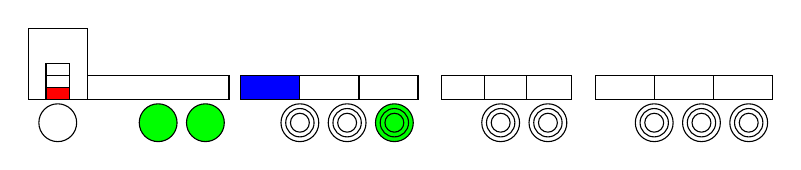
\begin{tikzpicture}[ scale=0.3]
				% Tractor
				\draw (7.5,2) rectangle (10,5);
				\draw[fill=red] (8.25,2) rectangle (9.25,2.5);
				\draw (8.25,2.5) rectangle (9.25,3);
				\draw (8.25,3) rectangle (9.25,3.5);
				\draw (10,2) rectangle (16,3);
				\draw (8.75,1) circle (0.8);
				\draw[fill=green!100] (13,1) circle (0.8);
				\draw[fill=green!100] (15,1) circle (0.8);

				% Semi-trailer
				\draw[fill=blue] (16.5,2) rectangle (19,3);
				\draw (19,2) rectangle (21.5,3);
				\draw (21.5,2) rectangle (24,3);
				% \draw (17,0.5) rectangle (18,1);
				% \draw (17,1) rectangle (18,1.5);
				% \draw (17,1.5) rectangle (18,2);
				\draw (19,1) circle (0.8);
				\draw (19,1) circle (0.6);
				\draw (19,1) circle (0.4);
				\draw (21,1) circle (0.8);
				\draw (21,1) circle (0.6);
				\draw (21,1) circle (0.4);	
				\draw[fill=green!100] (23,1) circle (0.8);
				\draw (23,1) circle (0.6);
				\draw (23,1) circle (0.4);

				% Dolly
				\draw (25,2) rectangle (26.8,3);
				\draw (26.8,2) rectangle (28.6,3);
				\draw (28.6,2) rectangle (30.5,3);
				% \draw (25.5,0.5) rectangle (26.5,1);
				% \draw (25.5,1) rectangle (26.5,1.5);
				% \draw (25.5,1.5) rectangle (26.5,2);
				\draw (27.5,1) circle (0.8);
				\draw (27.5,1) circle (0.6);
				\draw (27.5,1) circle (0.4);	
				\draw (29.5,1) circle (0.8);
				\draw (29.5,1) circle (0.6);
				\draw (29.5,1) circle (0.4);	

				% Semi-trailer
				\draw (31.5,2) rectangle (34,3);
				\draw (34,2) rectangle (36.5,3);
				\draw (36.5,2) rectangle (39,3);
				% \draw (32,0.5) rectangle (33,1);
				% \draw (32,1) rectangle (33,1.5);
				% \draw (32,1.5) rectangle (33,2);
				\draw (34,1) circle (0.8);
				\draw (34,1) circle (0.6);
				\draw (34,1) circle (0.4);
				\draw (36,1) circle (0.8);
				\draw (36,1) circle (0.6);
				\draw (36,1) circle (0.4);	
				\draw (38,1) circle (0.8);
				\draw (38,1) circle (0.6);
				\draw (38,1) circle (0.4);
			\end{tikzpicture} & 1.28676 \\

		70 & 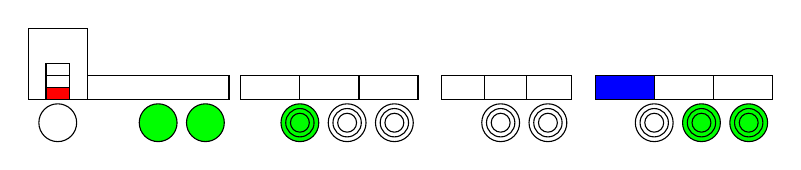
\begin{tikzpicture}[ scale=0.3]
				% Tractor
				\draw (7.5,2) rectangle (10,5);
				\draw[fill=red] (8.25,2) rectangle (9.25,2.5);
				\draw (8.25,2.5) rectangle (9.25,3);
				\draw (8.25,3) rectangle (9.25,3.5);
				\draw (10,2) rectangle (16,3);
				\draw (8.75,1) circle (0.8);
				\draw[fill=green!100] (13,1) circle (0.8);
				\draw[fill=green!100] (15,1) circle (0.8);

				% Semi-trailer
				\draw (16.5,2) rectangle (19,3);
				\draw (19,2) rectangle (21.5,3);
				\draw (21.5,2) rectangle (24,3);
				% \draw (17,0.5) rectangle (18,1);
				% \draw (17,1) rectangle (18,1.5);
				% \draw (17,1.5) rectangle (18,2);
				\draw[fill=green!100] (19,1) circle (0.8);
				\draw (19,1) circle (0.6);
				\draw (19,1) circle (0.4);
				\draw (21,1) circle (0.8);
				\draw (21,1) circle (0.6);
				\draw (21,1) circle (0.4);	
				\draw (23,1) circle (0.8);
				\draw (23,1) circle (0.6);
				\draw (23,1) circle (0.4);

				% Dolly
				\draw (25,2) rectangle (26.8,3);
				\draw (26.8,2) rectangle (28.6,3);
				\draw (28.6,2) rectangle (30.5,3);
				% \draw (25.5,0.5) rectangle (26.5,1);
				% \draw (25.5,1) rectangle (26.5,1.5);
				% \draw (25.5,1.5) rectangle (26.5,2);
				\draw (27.5,1) circle (0.8);
				\draw (27.5,1) circle (0.6);
				\draw (27.5,1) circle (0.4);	
				\draw (29.5,1) circle (0.8);
				\draw (29.5,1) circle (0.6);
				\draw (29.5,1) circle (0.4);	

				% Semi-trailer
				\draw[fill=blue] (31.5,2) rectangle (34,3);
				\draw (34,2) rectangle (36.5,3);
				\draw (36.5,2) rectangle (39,3);
				% \draw (32,0.5) rectangle (33,1);
				% \draw (32,1) rectangle (33,1.5);
				% \draw (32,1.5) rectangle (33,2);
				\draw (34,1) circle (0.8);
				\draw (34,1) circle (0.6);
				\draw (34,1) circle (0.4);
				\draw[fill=green!100] (36,1) circle (0.8);
				\draw (36,1) circle (0.6);
				\draw (36,1) circle (0.4);	
				\draw[fill=green!100] (38,1) circle (0.8);
				\draw (38,1) circle (0.6);
				\draw (38,1) circle (0.4);
			\end{tikzpicture} & 1.5351 \\
		
		80 & 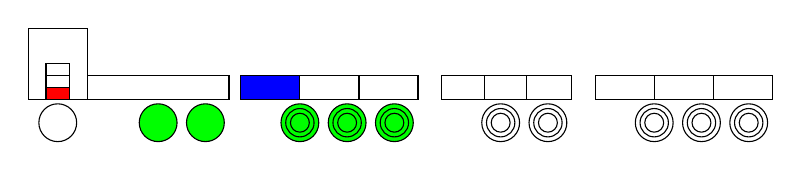
\begin{tikzpicture}[ scale=0.3]
				% Tractor
				\draw (7.5,2) rectangle (10,5);
				\draw[fill=red] (8.25,2) rectangle (9.25,2.5);
				\draw (8.25,2.5) rectangle (9.25,3);
				\draw (8.25,3) rectangle (9.25,3.5);
				\draw (10,2) rectangle (16,3);
				\draw (8.75,1) circle (0.8);
				\draw[fill=green!100] (13,1) circle (0.8);
				\draw[fill=green!100] (15,1) circle (0.8);

				% Semi-trailer
				\draw[fill=blue] (16.5,2) rectangle (19,3);
				\draw (19,2) rectangle (21.5,3);
				\draw (21.5,2) rectangle (24,3);
				% \draw (17,0.5) rectangle (18,1);
				% \draw (17,1) rectangle (18,1.5);
				% \draw (17,1.5) rectangle (18,2);
				\draw[fill=green!100] (19,1) circle (0.8);
				\draw (19,1) circle (0.6);
				\draw (19,1) circle (0.4);
				\draw[fill=green!100] (21,1) circle (0.8);
				\draw (21,1) circle (0.6);
				\draw (21,1) circle (0.4);	
				\draw[fill=green!100] (23,1) circle (0.8);
				\draw (23,1) circle (0.6);
				\draw (23,1) circle (0.4);

				% Dolly
				\draw (25,2) rectangle (26.8,3);
				\draw (26.8,2) rectangle (28.6,3);
				\draw (28.6,2) rectangle (30.5,3);
				% \draw (25.5,0.5) rectangle (26.5,1);
				% \draw (25.5,1) rectangle (26.5,1.5);
				% \draw (25.5,1.5) rectangle (26.5,2);
				\draw (27.5,1) circle (0.8);
				\draw (27.5,1) circle (0.6);
				\draw (27.5,1) circle (0.4);	
				\draw (29.5,1) circle (0.8);
				\draw (29.5,1) circle (0.6);
				\draw (29.5,1) circle (0.4);	

				% Semi-trailer
				\draw (31.5,2) rectangle (34,3);
				\draw (34,2) rectangle (36.5,3);
				\draw (36.5,2) rectangle (39,3);
				% \draw (32,0.5) rectangle (33,1);
				% \draw (32,1) rectangle (33,1.5);
				% \draw (32,1.5) rectangle (33,2);
				\draw (34,1) circle (0.8);
				\draw (34,1) circle (0.6);
				\draw (34,1) circle (0.4);
				\draw (36,1) circle (0.8);
				\draw (36,1) circle (0.6);
				\draw (36,1) circle (0.4);	
				\draw (38,1) circle (0.8);
				\draw (38,1) circle (0.6);
				\draw (38,1) circle (0.4);
			\end{tikzpicture} & 1.8501 \\
			\hline
		\end{tabular}
		\label{table:optVisComb2025}
	\end{table}

	\begin{table}[H]
		\caption{Optimal combination configurations - Year 2025}
		\centering
		\begin{tabular}{c c c c c c}
		\hline\hline
		GCW & \multicolumn{4}{c}{Optimal configuration} & Vehicle Productivity \\ \cline{2-5}
		(t) & Tractor & Semi-trailer & Dolly & Semi-trailer & (\euro/\euro)\\ 
		\hline
		50 & 100\textbackslash000\textbackslash011 & 001\textbackslash100\textbackslash100 & 100\textbackslash010\textbackslash00 & 100\textbackslash100\textbackslash000 & 0.984204 \\
		60 & 100\textbackslash000\textbackslash011 & 001\textbackslash100\textbackslash011 & 100\textbackslash100\textbackslash00 & 100\textbackslash001\textbackslash000 & 1.28676 \\
		70 & 100\textbackslash000\textbackslash011 & 001\textbackslash100\textbackslash000 & 100\textbackslash100\textbackslash00 & 001\textbackslash100\textbackslash011 & 1.5351 \\
		80 & 100\textbackslash000\textbackslash011 & 001\textbackslash100\textbackslash111 & 001\textbackslash010\textbackslash00 & 010\textbackslash100\textbackslash000 & 1.8501 \\
		\hline
		\end{tabular}
		\label{table:optComb2025}
	\end{table}

	\begin{table}[H]
		\caption{Optimal combination configurations - Year 2030}
		\centering
		\begin{tabular}{c c c}
		\hline\hline
		GCW & Optimal configuration & Vehicle Productivity \\  
		\hline
		50 & 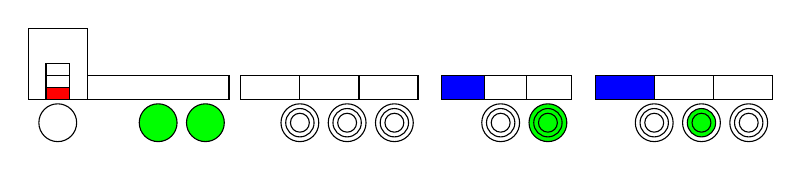
\begin{tikzpicture}[ scale=0.3]
				% Tractor
				\draw (7.5,2) rectangle (10,5);
				\draw[fill=red] (8.25,2) rectangle (9.25,2.5);
				\draw (8.25,2.5) rectangle (9.25,3);
				\draw (8.25,3) rectangle (9.25,3.5);
				\draw (10,2) rectangle (16,3);
				\draw (8.75,1) circle (0.8);
				\draw[fill=green!100] (13,1) circle (0.8);
				\draw[fill=green!100] (15,1) circle (0.8);

				% Semi-trailer
				\draw (16.5,2) rectangle (19,3);
				\draw (19,2) rectangle (21.5,3);
				\draw (21.5,2) rectangle (24,3);
				% \draw (17,0.5) rectangle (18,1);
				% \draw (17,1) rectangle (18,1.5);
				% \draw (17,1.5) rectangle (18,2);
				\draw (19,1) circle (0.8);
				\draw (19,1) circle (0.6);
				\draw (19,1) circle (0.4);
				\draw (21,1) circle (0.8);
				\draw (21,1) circle (0.6);
				\draw (21,1) circle (0.4);	
				\draw (23,1) circle (0.8);
				\draw (23,1) circle (0.6);
				\draw (23,1) circle (0.4);

				% Dolly
				\draw[fill=blue] (25,2) rectangle (26.8,3);
				\draw (26.8,2) rectangle (28.6,3);
				\draw (28.6,2) rectangle (30.5,3);
				% \draw (25.5,0.5) rectangle (26.5,1);
				% \draw (25.5,1) rectangle (26.5,1.5);
				% \draw (25.5,1.5) rectangle (26.5,2);
				\draw (27.5,1) circle (0.8);
				\draw (27.5,1) circle (0.6);
				\draw (27.5,1) circle (0.4);	
				\draw[fill=green!100] (29.5,1) circle (0.8);
				\draw (29.5,1) circle (0.6);
				\draw (29.5,1) circle (0.4);	

				% Semi-trailer
				\draw[fill=blue] (31.5,2) rectangle (34,3);
				\draw (34,2) rectangle (36.5,3);
				\draw (36.5,2) rectangle (39,3);
				% \draw (32,0.5) rectangle (33,1);
				% \draw (32,1) rectangle (33,1.5);
				% \draw (32,1.5) rectangle (33,2);
				\draw (34,1) circle (0.8);
				\draw (34,1) circle (0.6);
				\draw (34,1) circle (0.4);
				\draw (36,1) circle (0.8);
				\draw[fill=green!100] (36,1) circle (0.6);
				\draw (36,1) circle (0.4);	
				\draw (38,1) circle (0.8);
				\draw (38,1) circle (0.6);
				\draw (38,1) circle (0.4);
			\end{tikzpicture} & 0.99445 \\

		60 & 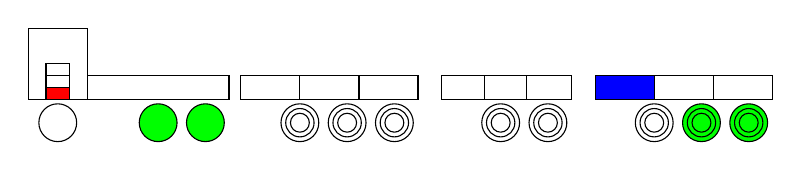
\begin{tikzpicture}[ scale=0.3]
				% Tractor
				\draw (7.5,2) rectangle (10,5);
				\draw[fill=red] (8.25,2) rectangle (9.25,2.5);
				\draw (8.25,2.5) rectangle (9.25,3);
				\draw (8.25,3) rectangle (9.25,3.5);
				\draw (10,2) rectangle (16,3);
				\draw (8.75,1) circle (0.8);
				\draw[fill=green!100] (13,1) circle (0.8);
				\draw[fill=green!100] (15,1) circle (0.8);

				% Semi-trailer
				\draw (16.5,2) rectangle (19,3);
				\draw (19,2) rectangle (21.5,3);
				\draw (21.5,2) rectangle (24,3);
				% \draw (17,0.5) rectangle (18,1);
				% \draw (17,1) rectangle (18,1.5);
				% \draw (17,1.5) rectangle (18,2);
				\draw (19,1) circle (0.8);
				\draw (19,1) circle (0.6);
				\draw (19,1) circle (0.4);
				\draw (21,1) circle (0.8);
				\draw (21,1) circle (0.6);
				\draw (21,1) circle (0.4);	
				\draw (23,1) circle (0.8);
				\draw (23,1) circle (0.6);
				\draw (23,1) circle (0.4);

				% Dolly
				\draw (25,2) rectangle (26.8,3);
				\draw (26.8,2) rectangle (28.6,3);
				\draw (28.6,2) rectangle (30.5,3);
				% \draw (25.5,0.5) rectangle (26.5,1);
				% \draw (25.5,1) rectangle (26.5,1.5);
				% \draw (25.5,1.5) rectangle (26.5,2);
				\draw (27.5,1) circle (0.8);
				\draw (27.5,1) circle (0.6);
				\draw (27.5,1) circle (0.4);	
				\draw (29.5,1) circle (0.8);
				\draw (29.5,1) circle (0.6);
				\draw (29.5,1) circle (0.4);	

				% Semi-trailer
				\draw[fill=blue] (31.5,2) rectangle (34,3);
				\draw (34,2) rectangle (36.5,3);
				\draw (36.5,2) rectangle (39,3);
				% \draw (32,0.5) rectangle (33,1);
				% \draw (32,1) rectangle (33,1.5);
				% \draw (32,1.5) rectangle (33,2);
				\draw (34,1) circle (0.8);
				\draw (34,1) circle (0.6);
				\draw (34,1) circle (0.4);
				\draw[fill=green!100] (36,1) circle (0.8);
				\draw (36,1) circle (0.6);
				\draw (36,1) circle (0.4);	
				\draw[fill=green!100] (38,1) circle (0.8);
				\draw (38,1) circle (0.6);
				\draw (38,1) circle (0.4);
			\end{tikzpicture} & 1.30212 \\

		70 & 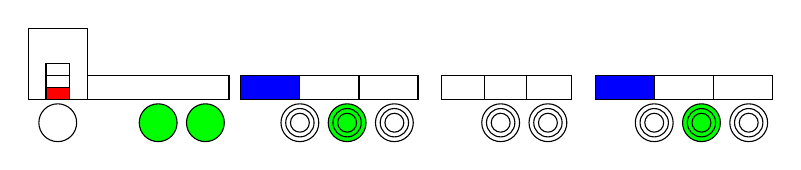
\begin{tikzpicture}[ scale=0.3]
				% Tractor
				\draw (7.5,2) rectangle (10,5);
				\draw[fill=red] (8.25,2) rectangle (9.25,2.5);
				\draw (8.25,2.5) rectangle (9.25,3);
				\draw (8.25,3) rectangle (9.25,3.5);
				\draw (10,2) rectangle (16,3);
				\draw (8.75,1) circle (0.8);
				\draw[fill=green!100] (13,1) circle (0.8);
				\draw[fill=green!100] (15,1) circle (0.8);

				% Semi-trailer
				\draw[fill=blue] (16.5,2) rectangle (19,3);
				\draw (19,2) rectangle (21.5,3);
				\draw (21.5,2) rectangle (24,3);
				% \draw (17,0.5) rectangle (18,1);
				% \draw (17,1) rectangle (18,1.5);
				% \draw (17,1.5) rectangle (18,2);
				\draw (19,1) circle (0.8);
				\draw (19,1) circle (0.6);
				\draw (19,1) circle (0.4);
				\draw[fill=green!100] (21,1) circle (0.8);
				\draw (21,1) circle (0.6);
				\draw (21,1) circle (0.4);	
				\draw (23,1) circle (0.8);
				\draw (23,1) circle (0.6);
				\draw (23,1) circle (0.4);

				% Dolly
				\draw (25,2) rectangle (26.8,3);
				\draw (26.8,2) rectangle (28.6,3);
				\draw (28.6,2) rectangle (30.5,3);
				% \draw (25.5,0.5) rectangle (26.5,1);
				% \draw (25.5,1) rectangle (26.5,1.5);
				% \draw (25.5,1.5) rectangle (26.5,2);
				\draw (27.5,1) circle (0.8);
				\draw (27.5,1) circle (0.6);
				\draw (27.5,1) circle (0.4);	
				\draw (29.5,1) circle (0.8);
				\draw (29.5,1) circle (0.6);
				\draw (29.5,1) circle (0.4);	

				% Semi-trailer
				\draw[fill=blue] (31.5,2) rectangle (34,3);
				\draw (34,2) rectangle (36.5,3);
				\draw (36.5,2) rectangle (39,3);
				% \draw (32,0.5) rectangle (33,1);
				% \draw (32,1) rectangle (33,1.5);
				% \draw (32,1.5) rectangle (33,2);
				\draw (34,1) circle (0.8);
				\draw (34,1) circle (0.6);
				\draw (34,1) circle (0.4);
				\draw[fill=green!100] (36,1) circle (0.8);
				\draw (36,1) circle (0.6);
				\draw (36,1) circle (0.4);	
				\draw (38,1) circle (0.8);
				\draw (38,1) circle (0.6);
				\draw (38,1) circle (0.4);
			\end{tikzpicture} & 1.55402 \\
		
		80 & 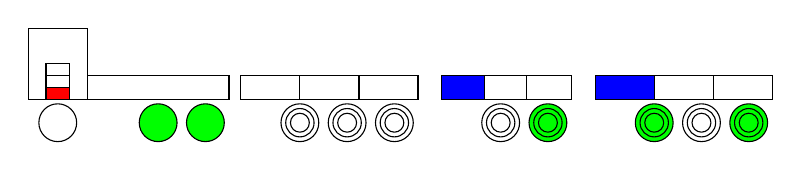
\begin{tikzpicture}[ scale=0.3]
				% Tractor
				\draw (7.5,2) rectangle (10,5);
				\draw[fill=red] (8.25,2) rectangle (9.25,2.5);
				\draw (8.25,2.5) rectangle (9.25,3);
				\draw (8.25,3) rectangle (9.25,3.5);
				\draw (10,2) rectangle (16,3);
				\draw (8.75,1) circle (0.8);
				\draw[fill=green!100] (13,1) circle (0.8);
				\draw[fill=green!100] (15,1) circle (0.8);

				% Semi-trailer
				\draw (16.5,2) rectangle (19,3);
				\draw (19,2) rectangle (21.5,3);
				\draw (21.5,2) rectangle (24,3);
				% \draw (17,0.5) rectangle (18,1);
				% \draw (17,1) rectangle (18,1.5);
				% \draw (17,1.5) rectangle (18,2);
				\draw (19,1) circle (0.8);
				\draw (19,1) circle (0.6);
				\draw (19,1) circle (0.4);
				\draw (21,1) circle (0.8);
				\draw (21,1) circle (0.6);
				\draw (21,1) circle (0.4);	
				\draw (23,1) circle (0.8);
				\draw (23,1) circle (0.6);
				\draw (23,1) circle (0.4);

				% Dolly
				\draw[fill=blue] (25,2) rectangle (26.8,3);
				\draw (26.8,2) rectangle (28.6,3);
				\draw (28.6,2) rectangle (30.5,3);
				% \draw (25.5,0.5) rectangle (26.5,1);
				% \draw (25.5,1) rectangle (26.5,1.5);
				% \draw (25.5,1.5) rectangle (26.5,2);
				\draw (27.5,1) circle (0.8);
				\draw (27.5,1) circle (0.6);
				\draw (27.5,1) circle (0.4);	
				\draw[fill=green!100] (29.5,1) circle (0.8);
				\draw (29.5,1) circle (0.6);
				\draw (29.5,1) circle (0.4);	

				% Semi-trailer
				\draw[fill=blue] (31.5,2) rectangle (34,3);
				\draw (34,2) rectangle (36.5,3);
				\draw (36.5,2) rectangle (39,3);
				% \draw (32,0.5) rectangle (33,1);
				% \draw (32,1) rectangle (33,1.5);
				% \draw (32,1.5) rectangle (33,2);
				\draw[fill=green!100] (34,1) circle (0.8);
				\draw (34,1) circle (0.6);
				\draw (34,1) circle (0.4);
				\draw (36,1) circle (0.8);
				\draw (36,1) circle (0.6);
				\draw (36,1) circle (0.4);	
				\draw[fill=green!100] (38,1) circle (0.8);
				\draw (38,1) circle (0.6);
				\draw (38,1) circle (0.4);
			\end{tikzpicture} & 1.87496 \\
			\hline
		\end{tabular}
		\label{table:optVisComb2030}
	\end{table}

	\begin{table}[H]
		\caption{Optimal combination configurations - Year 2030}
		\centering
		\begin{tabular}{c c c c c c}
		\hline\hline
		GCW & \multicolumn{4}{c}{Optimal configuration} & Vehicle Productivity \\ \cline{2-5}
		(t) & Tractor & Semi-trailer & Dolly & Semi-trailer & (\euro/\euro)\\ 
		\hline
		50 & 100\textbackslash000\textbackslash011 & 100\textbackslash100\textbackslash000 & 001\textbackslash100\textbackslash01 & 001\textbackslash010\textbackslash000 & 0.99445 \\
		60 & 100\textbackslash000\textbackslash011 & 001\textbackslash100\textbackslash000 & 010\textbackslash100\textbackslash00 & 001\textbackslash100\textbackslash011 & 1.30212 \\
		70 & 100\textbackslash000\textbackslash011 & 001\textbackslash100\textbackslash010 & 001\textbackslash010\textbackslash00 & 001\textbackslash100\textbackslash010 & 1.55402 \\
		80 & 100\textbackslash000\textbackslash011 & 001\textbackslash010\textbackslash000 & 001\textbackslash100\textbackslash01 & 001\textbackslash100\textbackslash101 & 1.87496 \\
		\hline
		\end{tabular}
		\label{table:optComb2030}
	\end{table}

	As can be seen, the engine tends to be downsized from the D16 to the D13 and D11 variants complemented by increased axle electrification. An detailed analysis of the results follows.\\

\section{Comparison with conventional combinations}
	Combinations that are powered only by the engine are chosen as a 'base' variant and compared with the optimal configuration for each GCW across the years. As can be seen, the fuel savings resulting from axle electrification and comparatively smaller driver wages owing to shorter mission times consistently drive the productivity higher. For example, the optimal configuration for the 50t combination in the year 2015 is compared with the standard A-Double driven by the D16 engine variant. The fixed and variable costs are compared between the two combinations to motivate the increased mission productivity. As can be seen in Figure \ref{2015AC0vsAC1}, reduced fuel consumption in case of the D13 variant by 5\% as well as reduced powertrain prices by 2\% can be related to improvement in productivity by 3\%.\\

	\begin{figure}[H]
		\begin{subfigure}{0.5\textwidth}
			\centering
			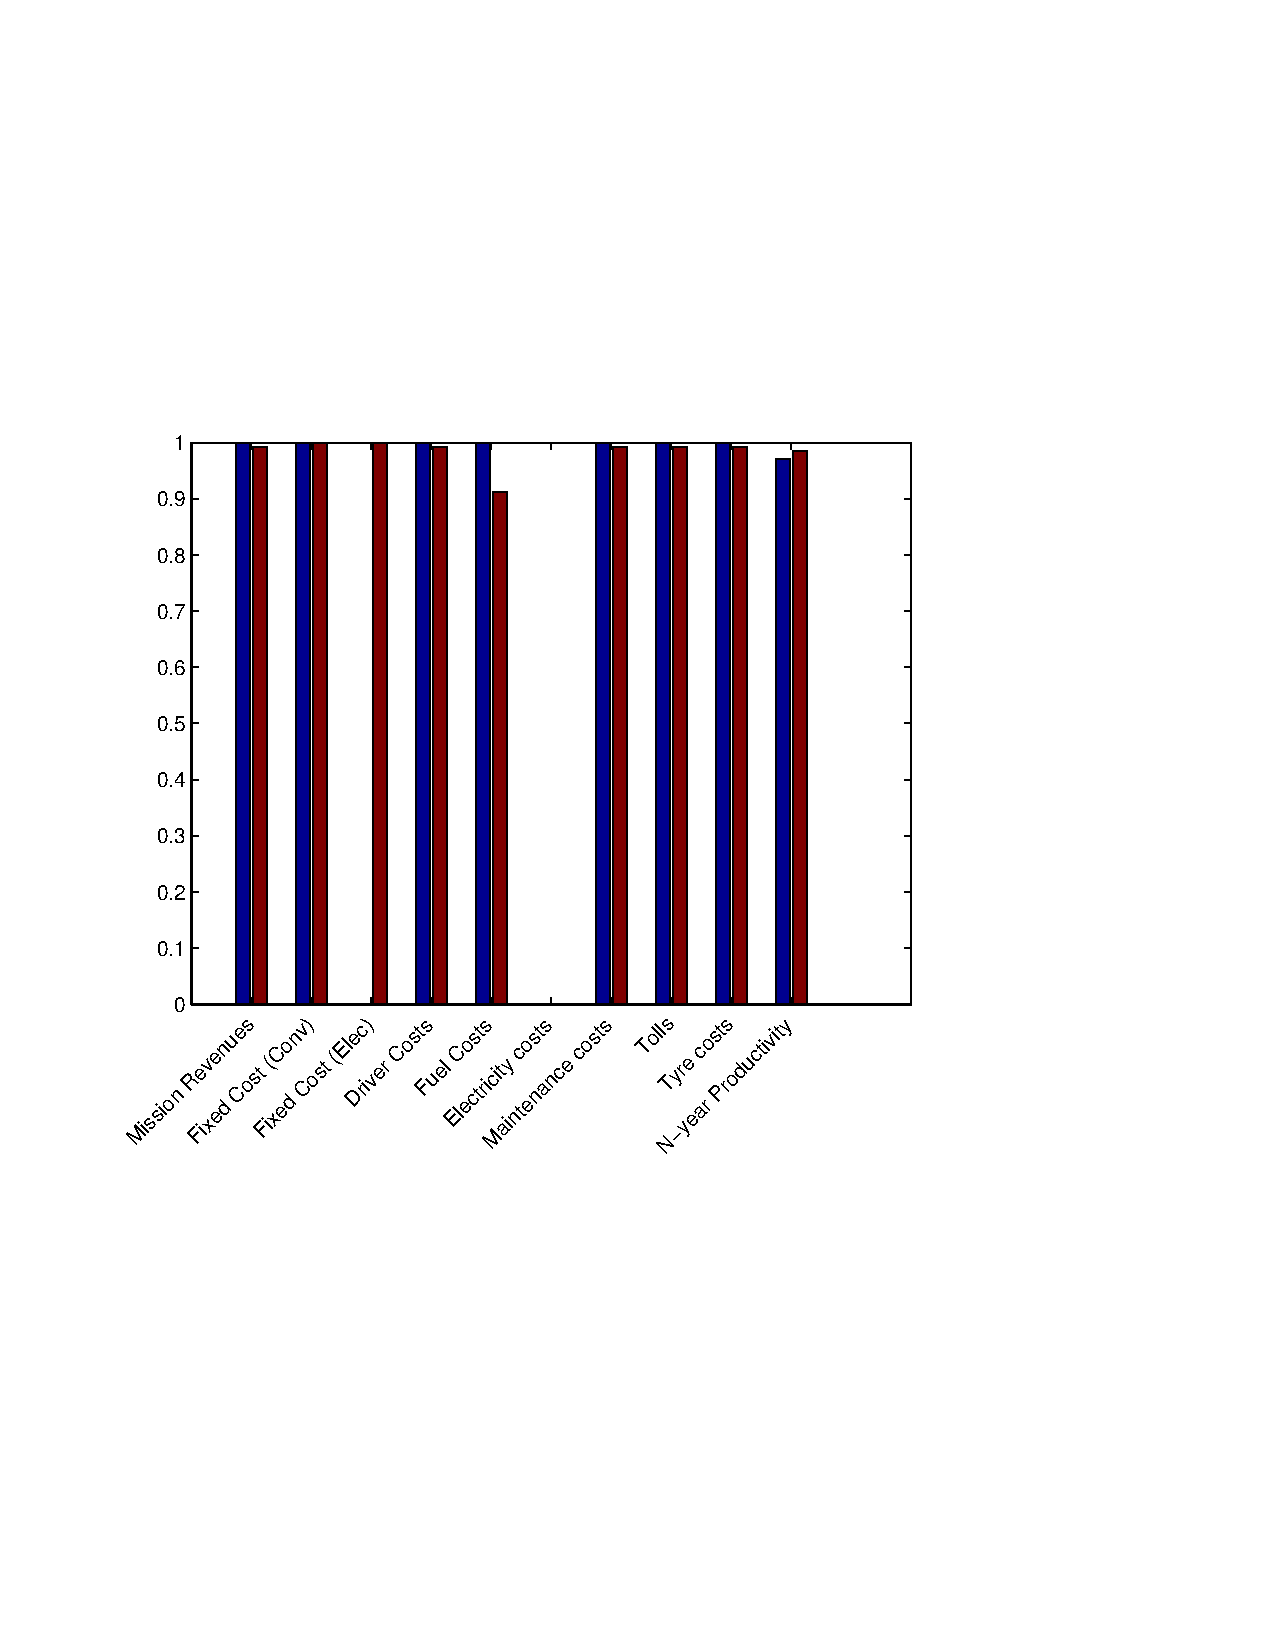
\includegraphics[width=\linewidth, clip=true, trim=45 225 135 208]{figures/OptimalCombinationResults/2015/A.pdf}
			\caption{GCW=50t}
		\end{subfigure}
		\begin{subfigure}{.5\textwidth}
			\centering
			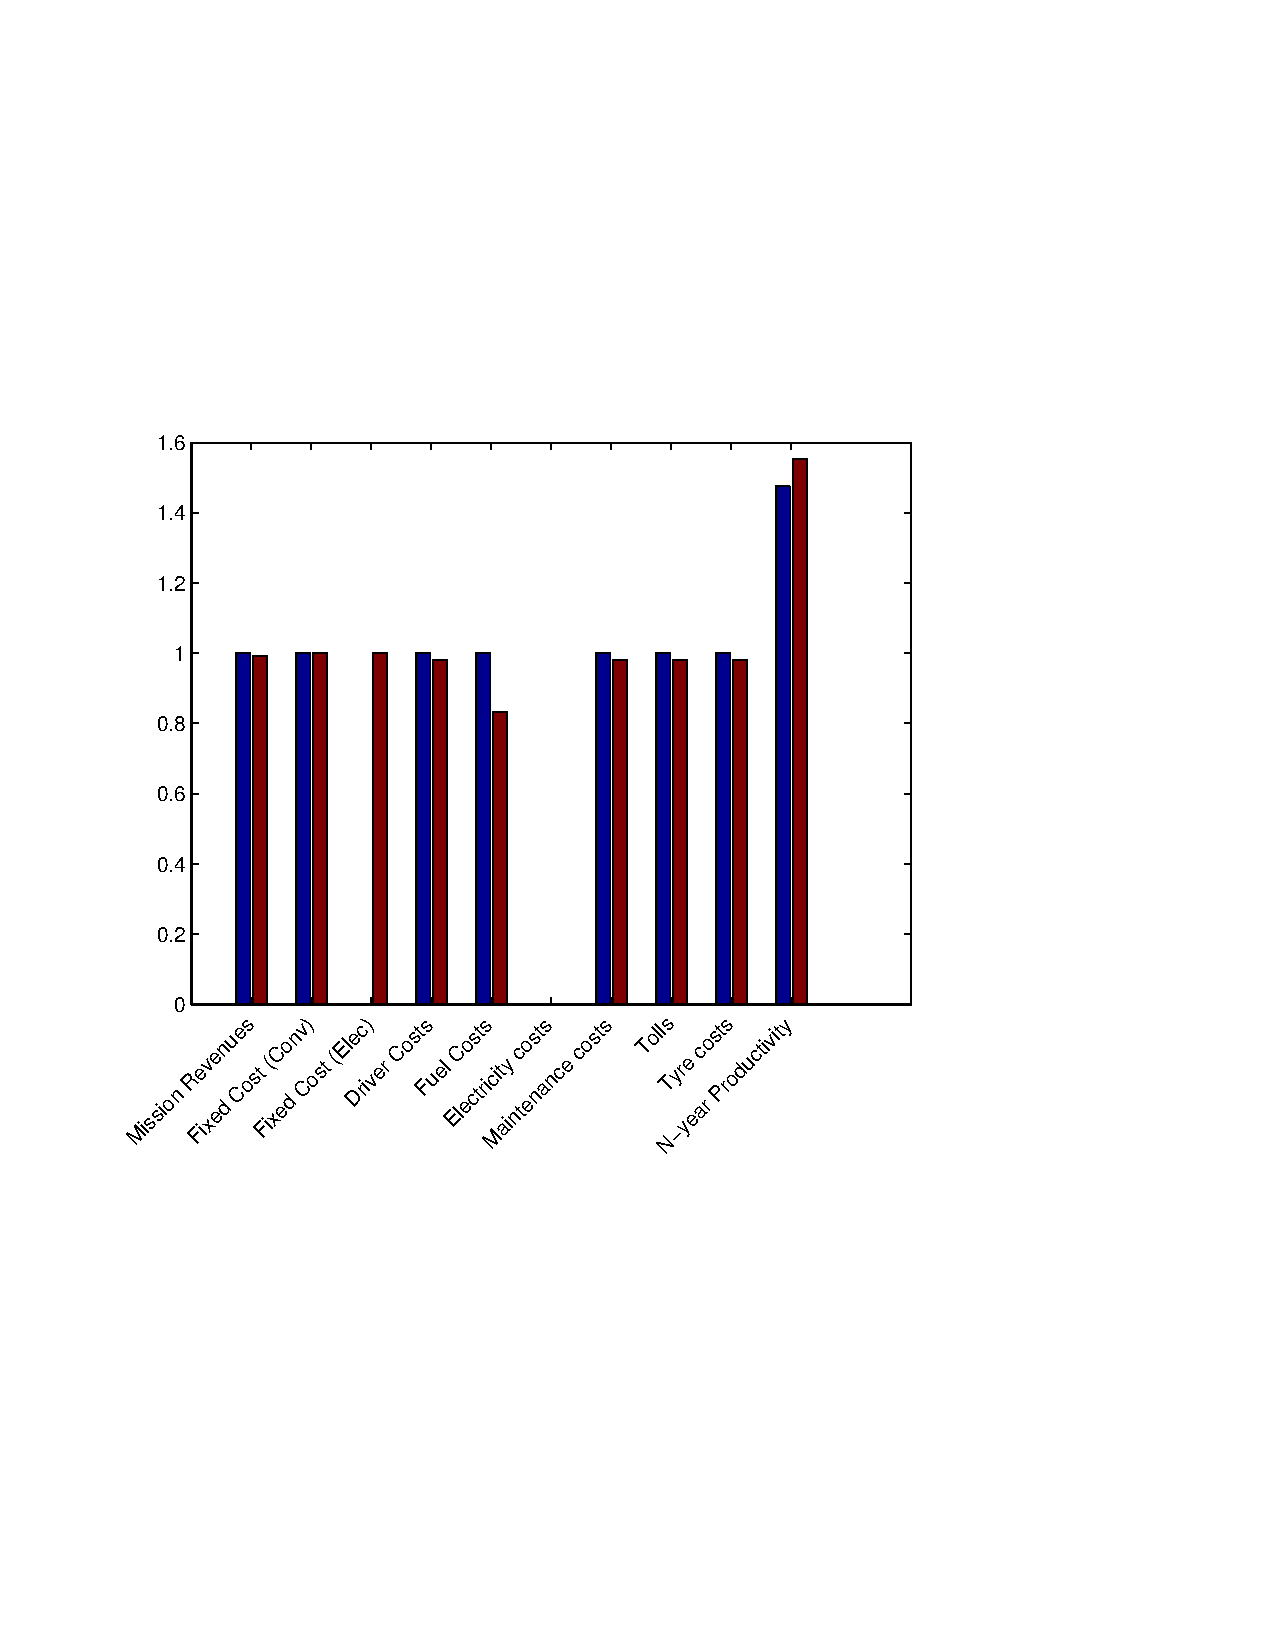
\includegraphics[width=\linewidth, clip=true, trim=45 225 135 208]{figures/OptimalCombinationResults/2020/C.pdf}
			\caption{GCW=70t}
		\end{subfigure}
		\caption{Optimal variant compared with the conventional combination}
		\label{2015AC0vsAC1}
	\end{figure}

\section{Optimal Combinations for increasing GCWs}
	The productivity performance of optimal configurations derived for varying GCWs in each year are observed and documented below. It can be seen in Figure \ref{prodVaryGCW2015} that optimal configurations for increasing GCWs show increased productivity. This implies that with increasing revenues, these optimal configurations bear the added advantage of reduced costs too.\\

	\begin{figure}[H]
		\centering
		\includegraphics[width=0.5\textwidth, clip=true, trim=45 225 125 208]{figures/OptimalCombinationResults/2015/Productivity.pdf}
		\caption{Variation of vehicle productivity with increasing GCW (2015)}
		\label{prodVaryGCW2015}
	\end{figure}

	The fixed and variable costs relative to the revenues earned for each GCW are depicted in Figure \ref{fixedVariableCostVaryGCW2015}. With increased electrification, the contribution of fixed electrification costs increases for the 70t optimal configuration compared to the 60t optimal configuration, and once again reduces for the optimal configuration for 80t. The general reduction in the revenue-to-electrification cost can be attributed to reduced net payload with increasing electrification. Increased revenue-to-driver wages with increasing GCWs are also indicative of higher average speeds relative to the freight transported. The same can be said of the revenue-to-fuel costs too.\\ 

	\begin{figure}[H]
		\begin{subfigure}{.5\textwidth}
			\centering
			\includegraphics[width=\linewidth, clip=true, trim=45 225 65 208]{figures/OptimalCombinationResults/2015/Fixed.pdf}
			\caption{Fixed costs}
		\end{subfigure}
		\begin{subfigure}{.5\textwidth}
			\centering
			\includegraphics[width=\linewidth, clip=true, trim=45 185 65 208]{figures/OptimalCombinationResults/2020/Variable.pdf}
			\caption{Driver \& Fuel costs}
		\end{subfigure}
		\caption{Variation of fixed and variable costs with increasing GCW (2015)}
		\label{fixedVariableCostVaryGCW2015}
	\end{figure}

	\newpage

	%Similar trends are observed in the fixed costs for varying GCWs as seen in Figure \ref{fixedCostVsGCWOverYears}.\\ 

	\begin{figure}[ht!]
		\begin{subfigure}{.5\textwidth}
			\centering
			\includegraphics[width=\linewidth, clip=true, trim=45 185 65 208]{figures/OptimalCombinationResults/2015/Fixed.pdf}
			\caption{Year 2015}
		\end{subfigure}
		\begin{subfigure}{.5\textwidth}
			\centering
			\includegraphics[width=\linewidth, clip=true, trim=45 185 65 208]{figures/OptimalCombinationResults/2020/Fixed.pdf}
			\caption{Year 2020}
		\end{subfigure}
		\begin{subfigure}{.5\textwidth}
			\centering
			\includegraphics[width=\linewidth, clip=true, trim=45 185 65 210]{figures/OptimalCombinationResults/2025/Fixed.pdf}
			\caption{Year 2025}
		\end{subfigure}
		\begin{subfigure}{.5\textwidth}
			\centering
			\includegraphics[width=\linewidth, clip=true, trim=45 185 65 210]{figures/OptimalCombinationResults/2030/Fixed.pdf}
			\caption{Year 2030}
		\end{subfigure}
		\caption{Variation of fixed costs with increasing GCW}
		\label{fixedCostVsGCWOverYears}
	\end{figure}

	\newpage

	\begin{figure}[ht!]
		\begin{subfigure}{.5\textwidth}
			\centering
			\includegraphics[width=\linewidth, clip=true, trim=45 185 65 208]{figures/OptimalCombinationResults/2015/Variable.pdf}
			\caption{Year 2015}
		\end{subfigure}
		\begin{subfigure}{.5\textwidth}
			\centering
			\includegraphics[width=\linewidth, clip=true, trim=45 185 65 208]{figures/OptimalCombinationResults/2020/Variable.pdf}
			\caption{Year 2020}
		\end{subfigure}
		\begin{subfigure}{.5\textwidth}
			\centering
			\includegraphics[width=\linewidth, clip=true, trim=45 185 65 210]{figures/OptimalCombinationResults/2025/Variable.pdf}
			\caption{Year 2025}
		\end{subfigure}
		\begin{subfigure}{.5\textwidth}
			\centering
			\includegraphics[width=\linewidth, clip=true, trim=45 185 65 210]{figures/OptimalCombinationResults/2030/Variable.pdf}
			\caption{Year 2030}
		\end{subfigure}
		\caption{Variation of driver and fuel costs with increasing GCW}
		\label{variableCostVsGCWOverYears}
	\end{figure}

	\newpage

\section{Optimal Combinations for constant GCW over the years}

	\begin{figure}[ht!]
		\centering
		\includegraphics[width=0.5\textwidth, clip=true, trim=45 225 125 208]{figures/OptimalCombinationResults/SingleGCW/A/Productivity.pdf}
		\caption{Variation of vehicle productivity for optimal solutions for constant GCW (2015-2030)}
		\label{prodConstGCWOverYears}
	\end{figure}

	The productivity characteristics of the optimal solutions derived for constant GCW from 2015 to 2030 is observed to increase consistently, albeit little. This can be seen in Figure \ref{prodConstGCWOverYears}. The miniscule increase in productivity can be attributed to the non-linear reduction in battery prices over the years as well as a sharper trend in fuel price rise.\\

	% \begin{table}[ht]
	% 	\caption{Optimal combination configurations - Year 2015}
	% 	\centering
	% 	\begin{tabular}{c c c}
	% 	\hline\hline
	% 	GCW & Optimal configuration & Vehicle Productivity \\  
	% 	\hline
	% 	50 & \begin{tikzpicture}[ scale=0.3]
	% 			% Tractor
	% 			\draw (7.5,2) rectangle (10,5);
	% 			\draw[fill=red] (8.25,2) rectangle (9.25,2.5);
	% 			\draw[fill=red] (8.25,2.5) rectangle (9.25,3);
	% 			\draw (8.25,3) rectangle (9.25,3.5);
	% 			\draw (10,2) rectangle (16,3);
	% 			\draw (8.75,1) circle (0.8);
	% 			\draw[fill=green!100] (13,1) circle (0.8);
	% 			\draw[fill=green!100] (15,1) circle (0.8);

	% 			% Semi-trailer
	% 			\draw (16.5,2) rectangle (24,3);
	% 			\draw (17,0.5) rectangle (18,1);
	% 			\draw (17,1) rectangle (18,1.5);
	% 			\draw (17,1.5) rectangle (18,2);
	% 			\draw (19,1) circle (0.8);
	% 			\draw (19,1) circle (0.6);
	% 			\draw (19,1) circle (0.4);
	% 			\draw (21,1) circle (0.8);
	% 			\draw (21,1) circle (0.6);
	% 			\draw (21,1) circle (0.4);	
	% 			\draw (23,1) circle (0.8);
	% 			\draw (23,1) circle (0.6);
	% 			\draw (23,1) circle (0.4);

	% 			% Dolly
	% 			\draw (25,2) rectangle (30.5,3);
	% 			\draw (25.5,0.5) rectangle (26.5,1);
	% 			\draw (25.5,1) rectangle (26.5,1.5);
	% 			\draw (25.5,1.5) rectangle (26.5,2);
	% 			\draw (27.5,1) circle (0.8);
	% 			\draw (27.5,1) circle (0.6);
	% 			\draw (27.5,1) circle (0.4);	
	% 			\draw (29.5,1) circle (0.8);
	% 			\draw (29.5,1) circle (0.6);
	% 			\draw (29.5,1) circle (0.4);	

	% 			% Semi-trailer
	% 			\draw (31.5,2) rectangle (39,3);
	% 			\draw (32,0.5) rectangle (33,1);
	% 			\draw (32,1) rectangle (33,1.5);
	% 			\draw (32,1.5) rectangle (33,2);
	% 			\draw (34,1) circle (0.8);
	% 			\draw (34,1) circle (0.6);
	% 			\draw (34,1) circle (0.4);
	% 			\draw (36,1) circle (0.8);
	% 			\draw (36,1) circle (0.6);
	% 			\draw (36,1) circle (0.4);	
	% 			\draw (38,1) circle (0.8);
	% 			\draw (38,1) circle (0.6);
	% 			\draw (38,1) circle (0.4);
	% 		\end{tikzpicture} & 0.960028 \\

	% 	60 & \begin{tikzpicture}[ scale=0.3]
	% 			% Tractor
	% 			\draw (7.5,2) rectangle (10,5);
	% 			\draw[fill=red] (8.25,2) rectangle (9.25,2.5);
	% 			\draw (8.25,2.5) rectangle (9.25,3);
	% 			\draw (8.25,3) rectangle (9.25,3.5);
	% 			\draw (10,2) rectangle (16,3);
	% 			\draw (8.75,1) circle (0.8);
	% 			\draw[fill=green!100] (13,1) circle (0.8);
	% 			\draw[fill=green!100] (15,1) circle (0.8);

	% 			% Semi-trailer
	% 			\draw (16.5,2) rectangle (24,3);
	% 			\draw (17,0.5) rectangle (18,1);
	% 			\draw (17,1) rectangle (18,1.5);
	% 			\draw[fill=blue] (17,1.5) rectangle (18,2);
	% 			\draw (19,1) circle (0.8);
	% 			\draw (19,1) circle (0.6);
	% 			\draw (19,1) circle (0.4);
	% 			\draw (21,1) circle (0.8);
	% 			\draw (21,1) circle (0.6);
	% 			\draw (21,1) circle (0.4);	
	% 			\draw[fill=green!100] (23,1) circle (0.8);
	% 			\draw (23,1) circle (0.6);
	% 			\draw (23,1) circle (0.4);

	% 			% Dolly
	% 			\draw (25,2) rectangle (30.5,3);
	% 			\draw (25.5,0.5) rectangle (26.5,1);
	% 			\draw (25.5,1) rectangle (26.5,1.5);
	% 			\draw (25.5,1.5) rectangle (26.5,2);
	% 			\draw (27.5,1) circle (0.8);
	% 			\draw (27.5,1) circle (0.6);
	% 			\draw (27.5,1) circle (0.4);	
	% 			\draw (29.5,1) circle (0.8);
	% 			\draw (29.5,1) circle (0.6);
	% 			\draw (29.5,1) circle (0.4);	

	% 			% Semi-trailer
	% 			\draw (31.5,2) rectangle (39,3);
	% 			\draw (32,0.5) rectangle (33,1);
	% 			\draw (32,1) rectangle (33,1.5);
	% 			\draw (32,1.5) rectangle (33,2);
	% 			\draw (34,1) circle (0.8);
	% 			\draw (34,1) circle (0.6);
	% 			\draw (34,1) circle (0.4);
	% 			\draw (36,1) circle (0.8);
	% 			\draw (36,1) circle (0.6);
	% 			\draw (36,1) circle (0.4);	
	% 			\draw (38,1) circle (0.8);
	% 			\draw (38,1) circle (0.6);
	% 			\draw (38,1) circle (0.4);
	% 		\end{tikzpicture} & 1.25954 \\

	% 	70 & \begin{tikzpicture}[ scale=0.3]
	% 			% Tractor
	% 			\draw (7.5,2) rectangle (10,5);
	% 			\draw[fill=red] (8.25,2) rectangle (9.25,2.5);
	% 			\draw (8.25,2.5) rectangle (9.25,3);
	% 			\draw (8.25,3) rectangle (9.25,3.5);
	% 			\draw (10,2) rectangle (16,3);
	% 			\draw (8.75,1) circle (0.8);
	% 			\draw[fill=green!100] (13,1) circle (0.8);
	% 			\draw[fill=green!100] (15,1) circle (0.8);

	% 			% Semi-trailer
	% 			\draw (16.5,2) rectangle (24,3);
	% 			\draw (17,0.5) rectangle (18,1);
	% 			\draw (17,1) rectangle (18,1.5);
	% 			\draw[fill=blue] (17,1.5) rectangle (18,2);
	% 			\draw (19,1) circle (0.8);
	% 			\draw (19,1) circle (0.6);
	% 			\draw (19,1) circle (0.4);
	% 			\draw[fill=green!100] (21,1) circle (0.8);
	% 			\draw (21,1) circle (0.6);
	% 			\draw (21,1) circle (0.4);	
	% 			\draw[fill=green!100] (23,1) circle (0.8);
	% 			\draw (23,1) circle (0.6);
	% 			\draw (23,1) circle (0.4);

	% 			% Dolly
	% 			\draw (25,2) rectangle (30.5,3);
	% 			\draw (25.5,0.5) rectangle (26.5,1);
	% 			\draw (25.5,1) rectangle (26.5,1.5);
	% 			\draw (25.5,1.5) rectangle (26.5,2);
	% 			\draw (27.5,1) circle (0.8);
	% 			\draw (27.5,1) circle (0.6);
	% 			\draw (27.5,1) circle (0.4);	
	% 			\draw (29.5,1) circle (0.8);
	% 			\draw (29.5,1) circle (0.6);
	% 			\draw (29.5,1) circle (0.4);	

	% 			% Semi-trailer
	% 			\draw (31.5,2) rectangle (39,3);
	% 			\draw (32,0.5) rectangle (33,1);
	% 			\draw (32,1) rectangle (33,1.5);
	% 			\draw (32,1.5) rectangle (33,2);
	% 			\draw (34,1) circle (0.8);
	% 			\draw (34,1) circle (0.6);
	% 			\draw (34,1) circle (0.4);
	% 			\draw (36,1) circle (0.8);
	% 			\draw (36,1) circle (0.6);
	% 			\draw (36,1) circle (0.4);	
	% 			\draw (38,1) circle (0.8);
	% 			\draw (38,1) circle (0.6);
	% 			\draw (38,1) circle (0.4);
	% 		\end{tikzpicture} & 1.49906 \\
		
	% 	80 & \begin{tikzpicture}[ scale=0.3]
	% 			% Tractor
	% 			\draw (7.5,2) rectangle (10,5);
	% 			\draw[fill=red] (8.25,2) rectangle (9.25,2.5);
	% 			\draw (8.25,2.5) rectangle (9.25,3);
	% 			\draw (8.25,3) rectangle (9.25,3.5);
	% 			\draw (10,2) rectangle (16,3);
	% 			\draw (8.75,1) circle (0.8);
	% 			\draw[fill=green!100] (13,1) circle (0.8);
	% 			\draw[fill=green!100] (15,1) circle (0.8);

	% 			% Semi-trailer
	% 			\draw (16.5,2) rectangle (24,3);
	% 			\draw (17,0.5) rectangle (18,1);
	% 			\draw (17,1) rectangle (18,1.5);
	% 			\draw (17,1.5) rectangle (18,2);
	% 			\draw (19,1) circle (0.8);
	% 			\draw (19,1) circle (0.6);
	% 			\draw (19,1) circle (0.4);
	% 			\draw (21,1) circle (0.8);
	% 			\draw (21,1) circle (0.6);
	% 			\draw (21,1) circle (0.4);	
	% 			\draw (23,1) circle (0.8);
	% 			\draw (23,1) circle (0.6);
	% 			\draw (23,1) circle (0.4);

	% 			% Dolly
	% 			\draw (25,2) rectangle (30.5,3);
	% 			\draw (25.5,0.5) rectangle (26.5,1);
	% 			\draw (25.5,1) rectangle (26.5,1.5);
	% 			\draw (25.5,1.5) rectangle (26.5,2);
	% 			\draw (27.5,1) circle (0.8);
	% 			\draw (27.5,1) circle (0.6);
	% 			\draw (27.5,1) circle (0.4);	
	% 			\draw (29.5,1) circle (0.8);
	% 			\draw (29.5,1) circle (0.6);
	% 			\draw (29.5,1) circle (0.4);	

	% 			% Semi-trailer
	% 			\draw (31.5,2) rectangle (39,3);
	% 			\draw (32,0.5) rectangle (33,1);
	% 			\draw (32,1) rectangle (33,1.5);
	% 			\draw[fill=blue] (32,1.5) rectangle (33,2);
	% 			\draw (34,1) circle (0.8);
	% 			\draw (34,1) circle (0.6);
	% 			\draw (34,1) circle (0.4);
	% 			\draw[fill=green!100] (36,1) circle (0.8);
	% 			\draw (36,1) circle (0.6);
	% 			\draw (36,1) circle (0.4);	
	% 			\draw[fill=green!100] (38,1) circle (0.8);
	% 			\draw (38,1) circle (0.6);
	% 			\draw (38,1) circle (0.4);
	% 		\end{tikzpicture} & 1.80818 \\

	% 	% 80 & 100\textbackslash000\textbackslash011 &
	% 	% 	 100\textbackslash010\textbackslash000 & 100\textbackslash100\textbackslash00 &
	% 	% 	 001\textbackslash100\textbackslash011 &  \\
	% 	\end{tabular}
	% 	\label{table:optComb2015}
	% \end{table}

\end{document}